O código XorShift é baseado em mudanças de posição nos bits ou bit shifts. O algoritmo implementado usa a operação de shift para fazer três movimentações nos bits do valor binário da semente, em seguida soma o resultado de tais shifts a um incremento, também advindo da semente somada ao valor Long 123456789L, e faz sua divisão pelo valor máx(número máximo de bits do valor “randomizado”) pela operação \%(módulo), a fim de entregar o resto da divisão como valor final. Caso o valor seja negativo, ele é multiplicado por -1 antes de ser retornado.
\\
Abaixo segue o código implementado:
\begin{figure}[H]
            \centering
                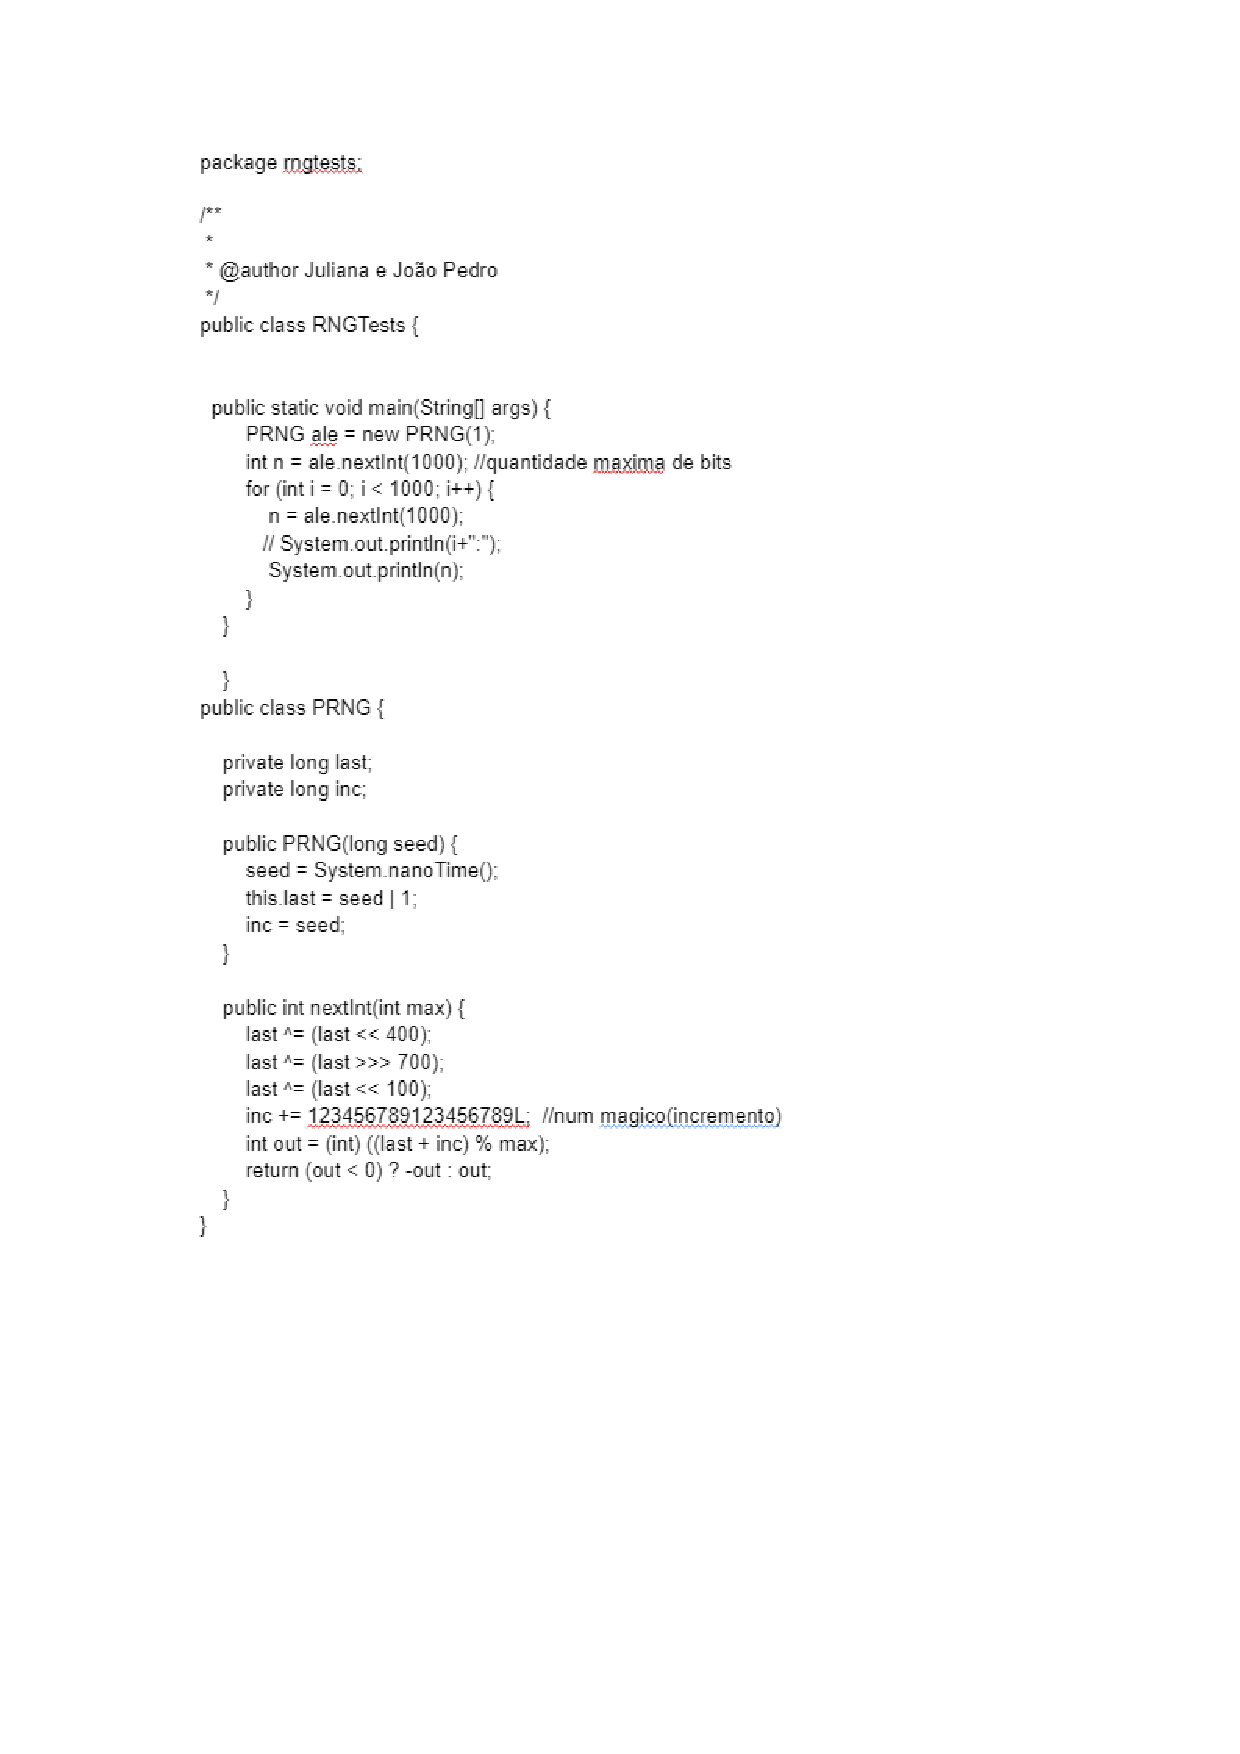
\includegraphics[width=0.72\textwidth]{codigorandom1.pdf}
                \caption{XorShift produzido}
                \label{fig:Desempenho}
        \end{figure} 
A fim de responder a pergunta “O que difere o algoritmo em estudo do Java.util.Random”, devemos compará-los.

O algoritmo da biblioteca java combina o código de gerador do tipo Xorshift com um gerador congruencial a fim de diversificar os resultados o máximo possível:

\begin{figure}[H]
            \centering
                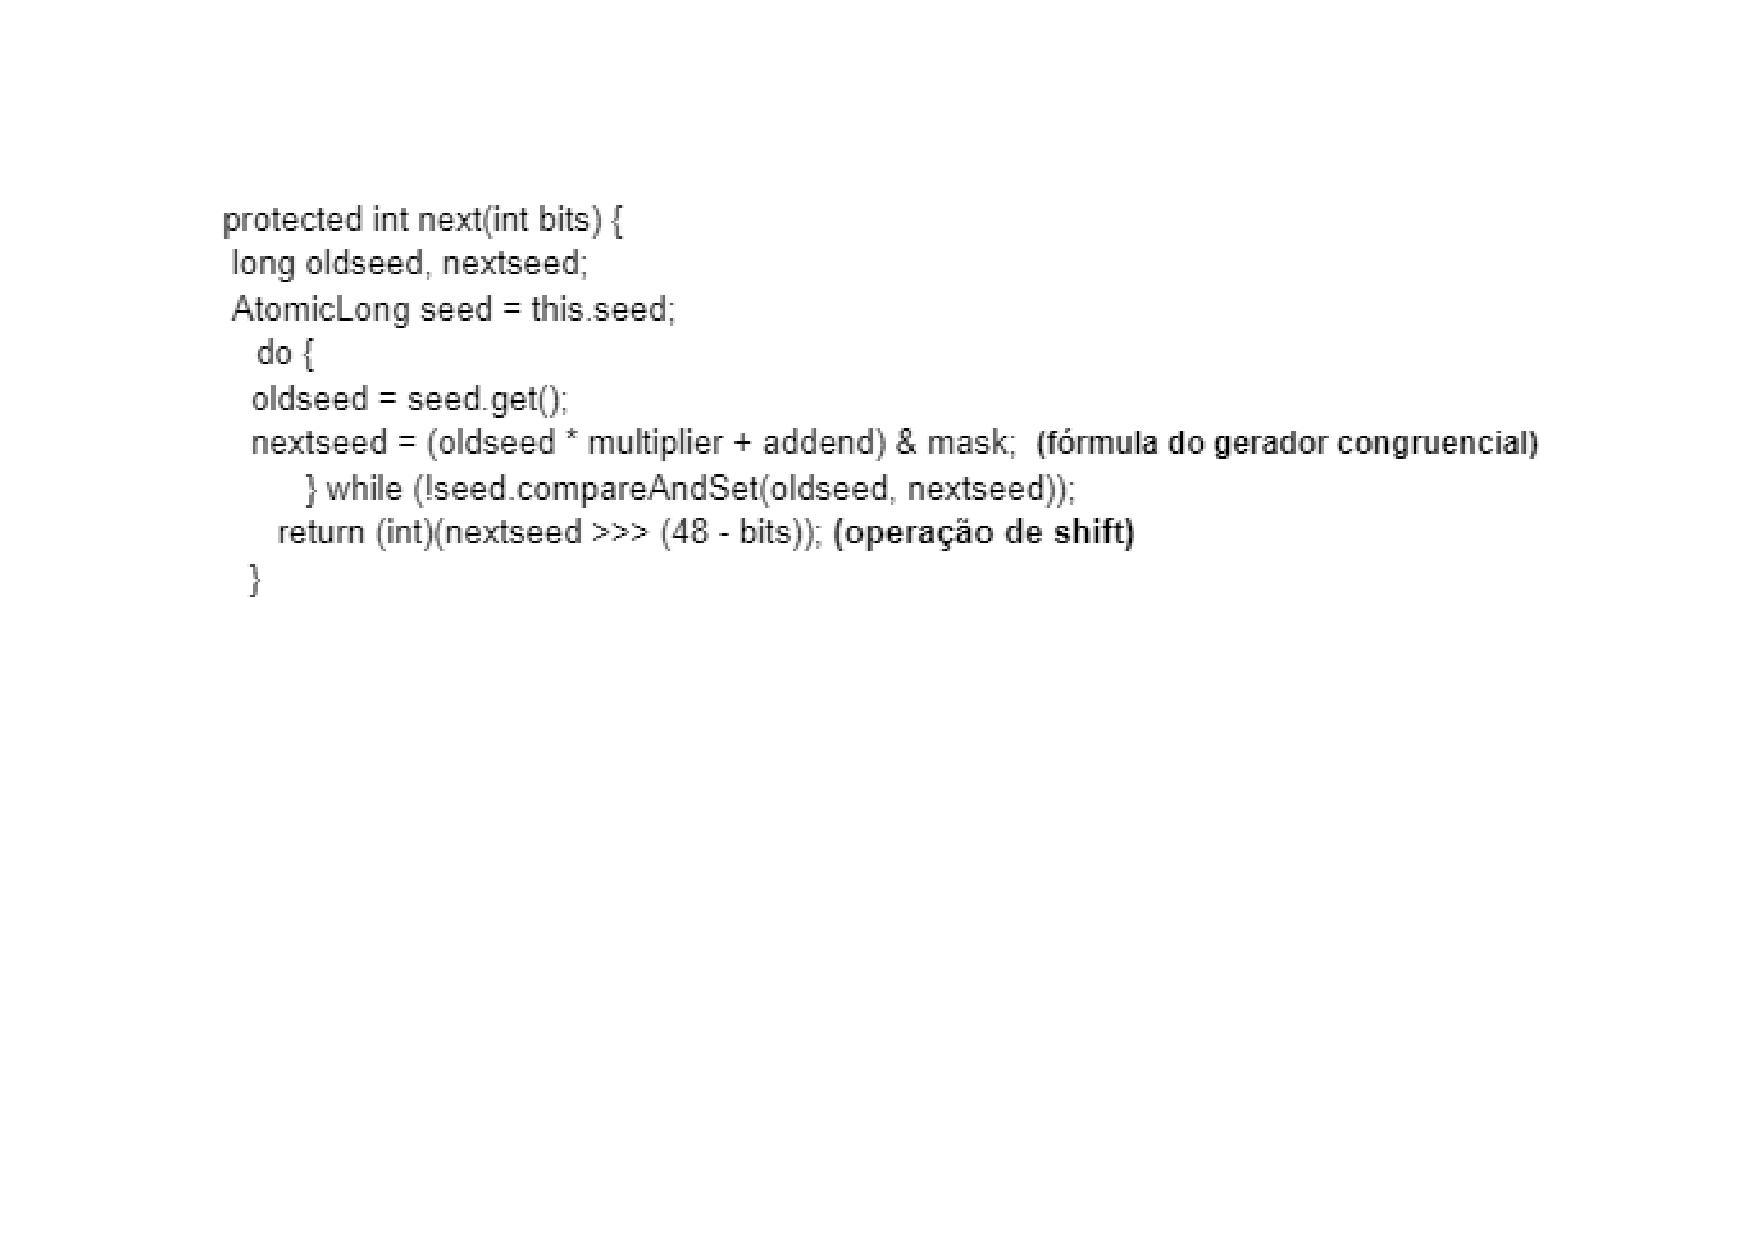
\includegraphics[width=0.74\textwidth]{codigorandomjava.pdf}
                 \caption{Java.util.Random(Gerador pseudo aleatório)}
                \label{fig:Desempenho}
        \end{figure} 

Ambos utilizam como seed(semente) o valor obtido usando System.nanoTime. O código implementado tem ordem de complexidade de tempo O(n) já que executa as chamadas de uma função  O(1)  n vezes dentro de um “for”. O código util.Random do java tem complexidade de O(1) por fazer chamadas do método nextInt que também é O(1) -ele só é executado uma vez, a não ser que o valor resultante seja igual à semente que o originou-, se for utilizado também n  vezes em um laço de repetição, terá também complexidade O(n), logo suas complexidades de tempo são iguais.
Após testes imprimindo vários valores com o loop até o algoritmo começar a repetir uma mesma sequência “randomizada”, encontramos o período de 144 com a execução do código xorshift, o que é igual a $2^{7}$+16, enquanto segundo a wikipédia \cite{SitWik} o período do algoritmo util.Random é de cerca de $2^{32}$ o que indica que o código util.Random pode retornar valores mais variados e menos previsíveis, devido ao período  maior de variabilidade antes de sofrer repetições garantidas.\cite{SitWik}\\       
\\
\\
\\
\\
\\
\\
\\
\\
\\
TABELA: XORSHIFT
\begin{figure}[H]
            \centering
                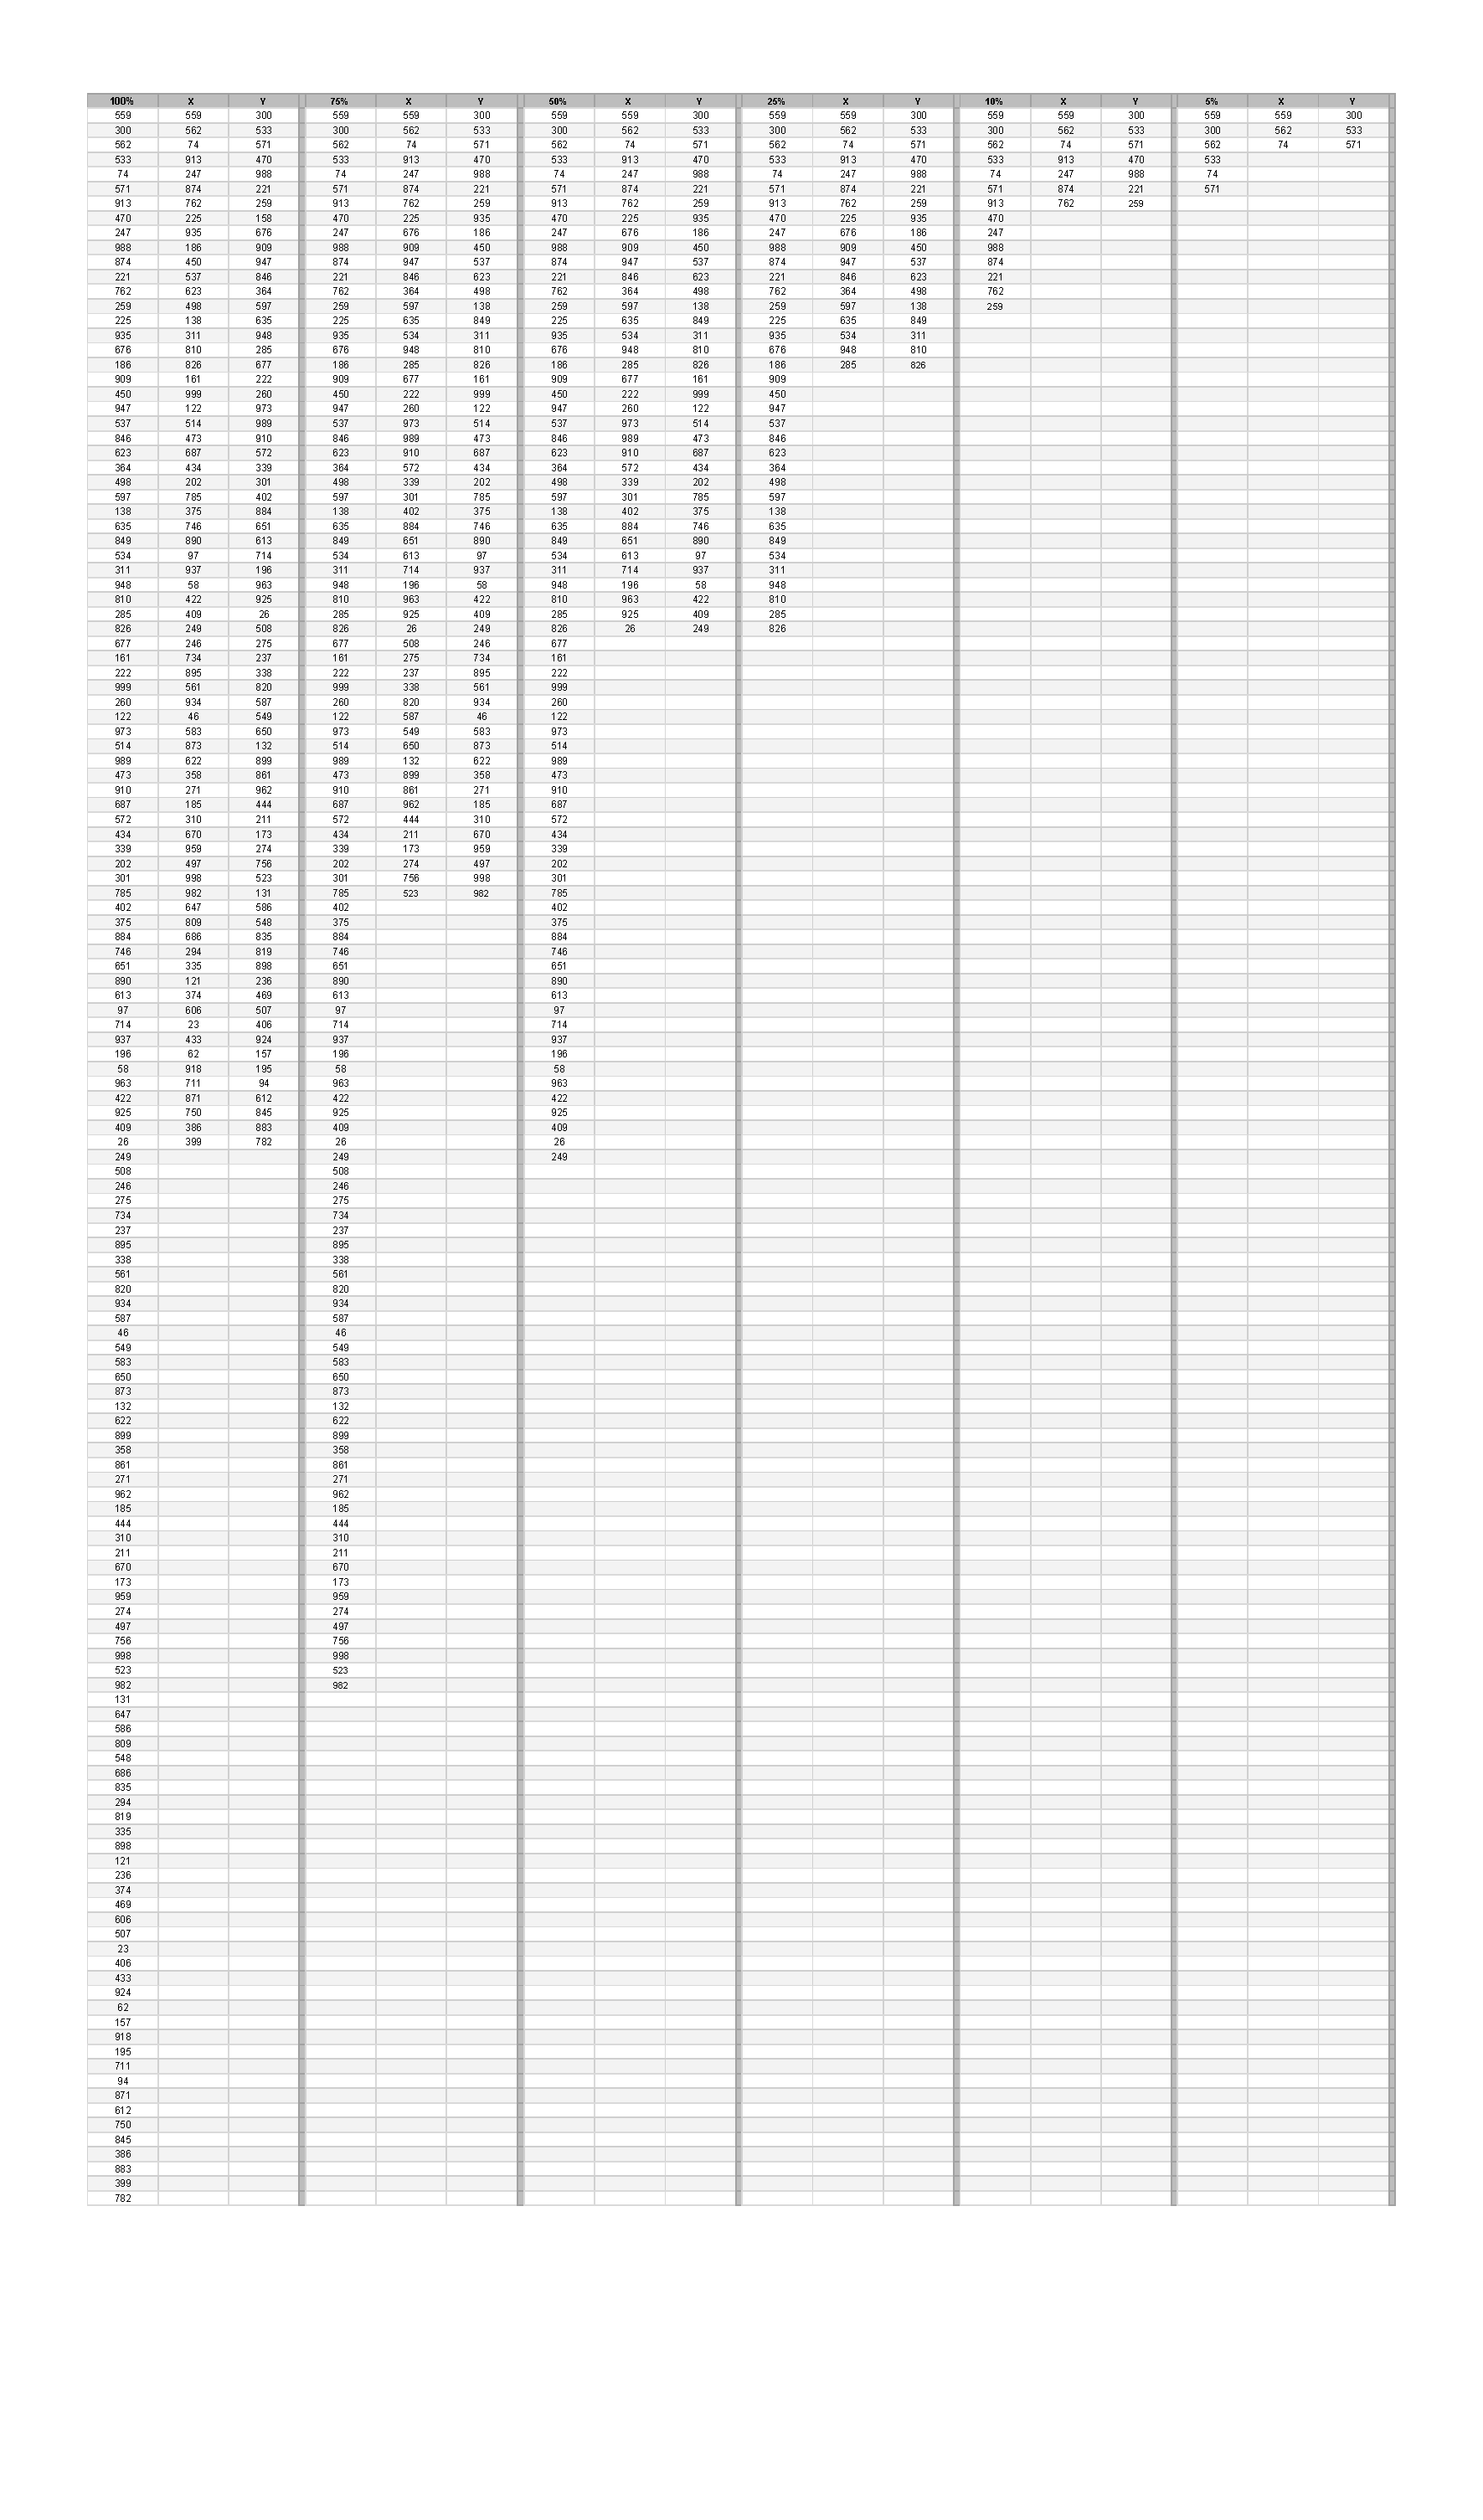
\includegraphics[width=0.84\textwidth]{tabelaExecXorShift.pdf}
                \caption{Valores obtidos em um período}
                \label{fig:Desempenho}
        \end{figure}

TABELA: JAVA.UTIL.RANDOM
\begin{figure}[H]
            \centering
                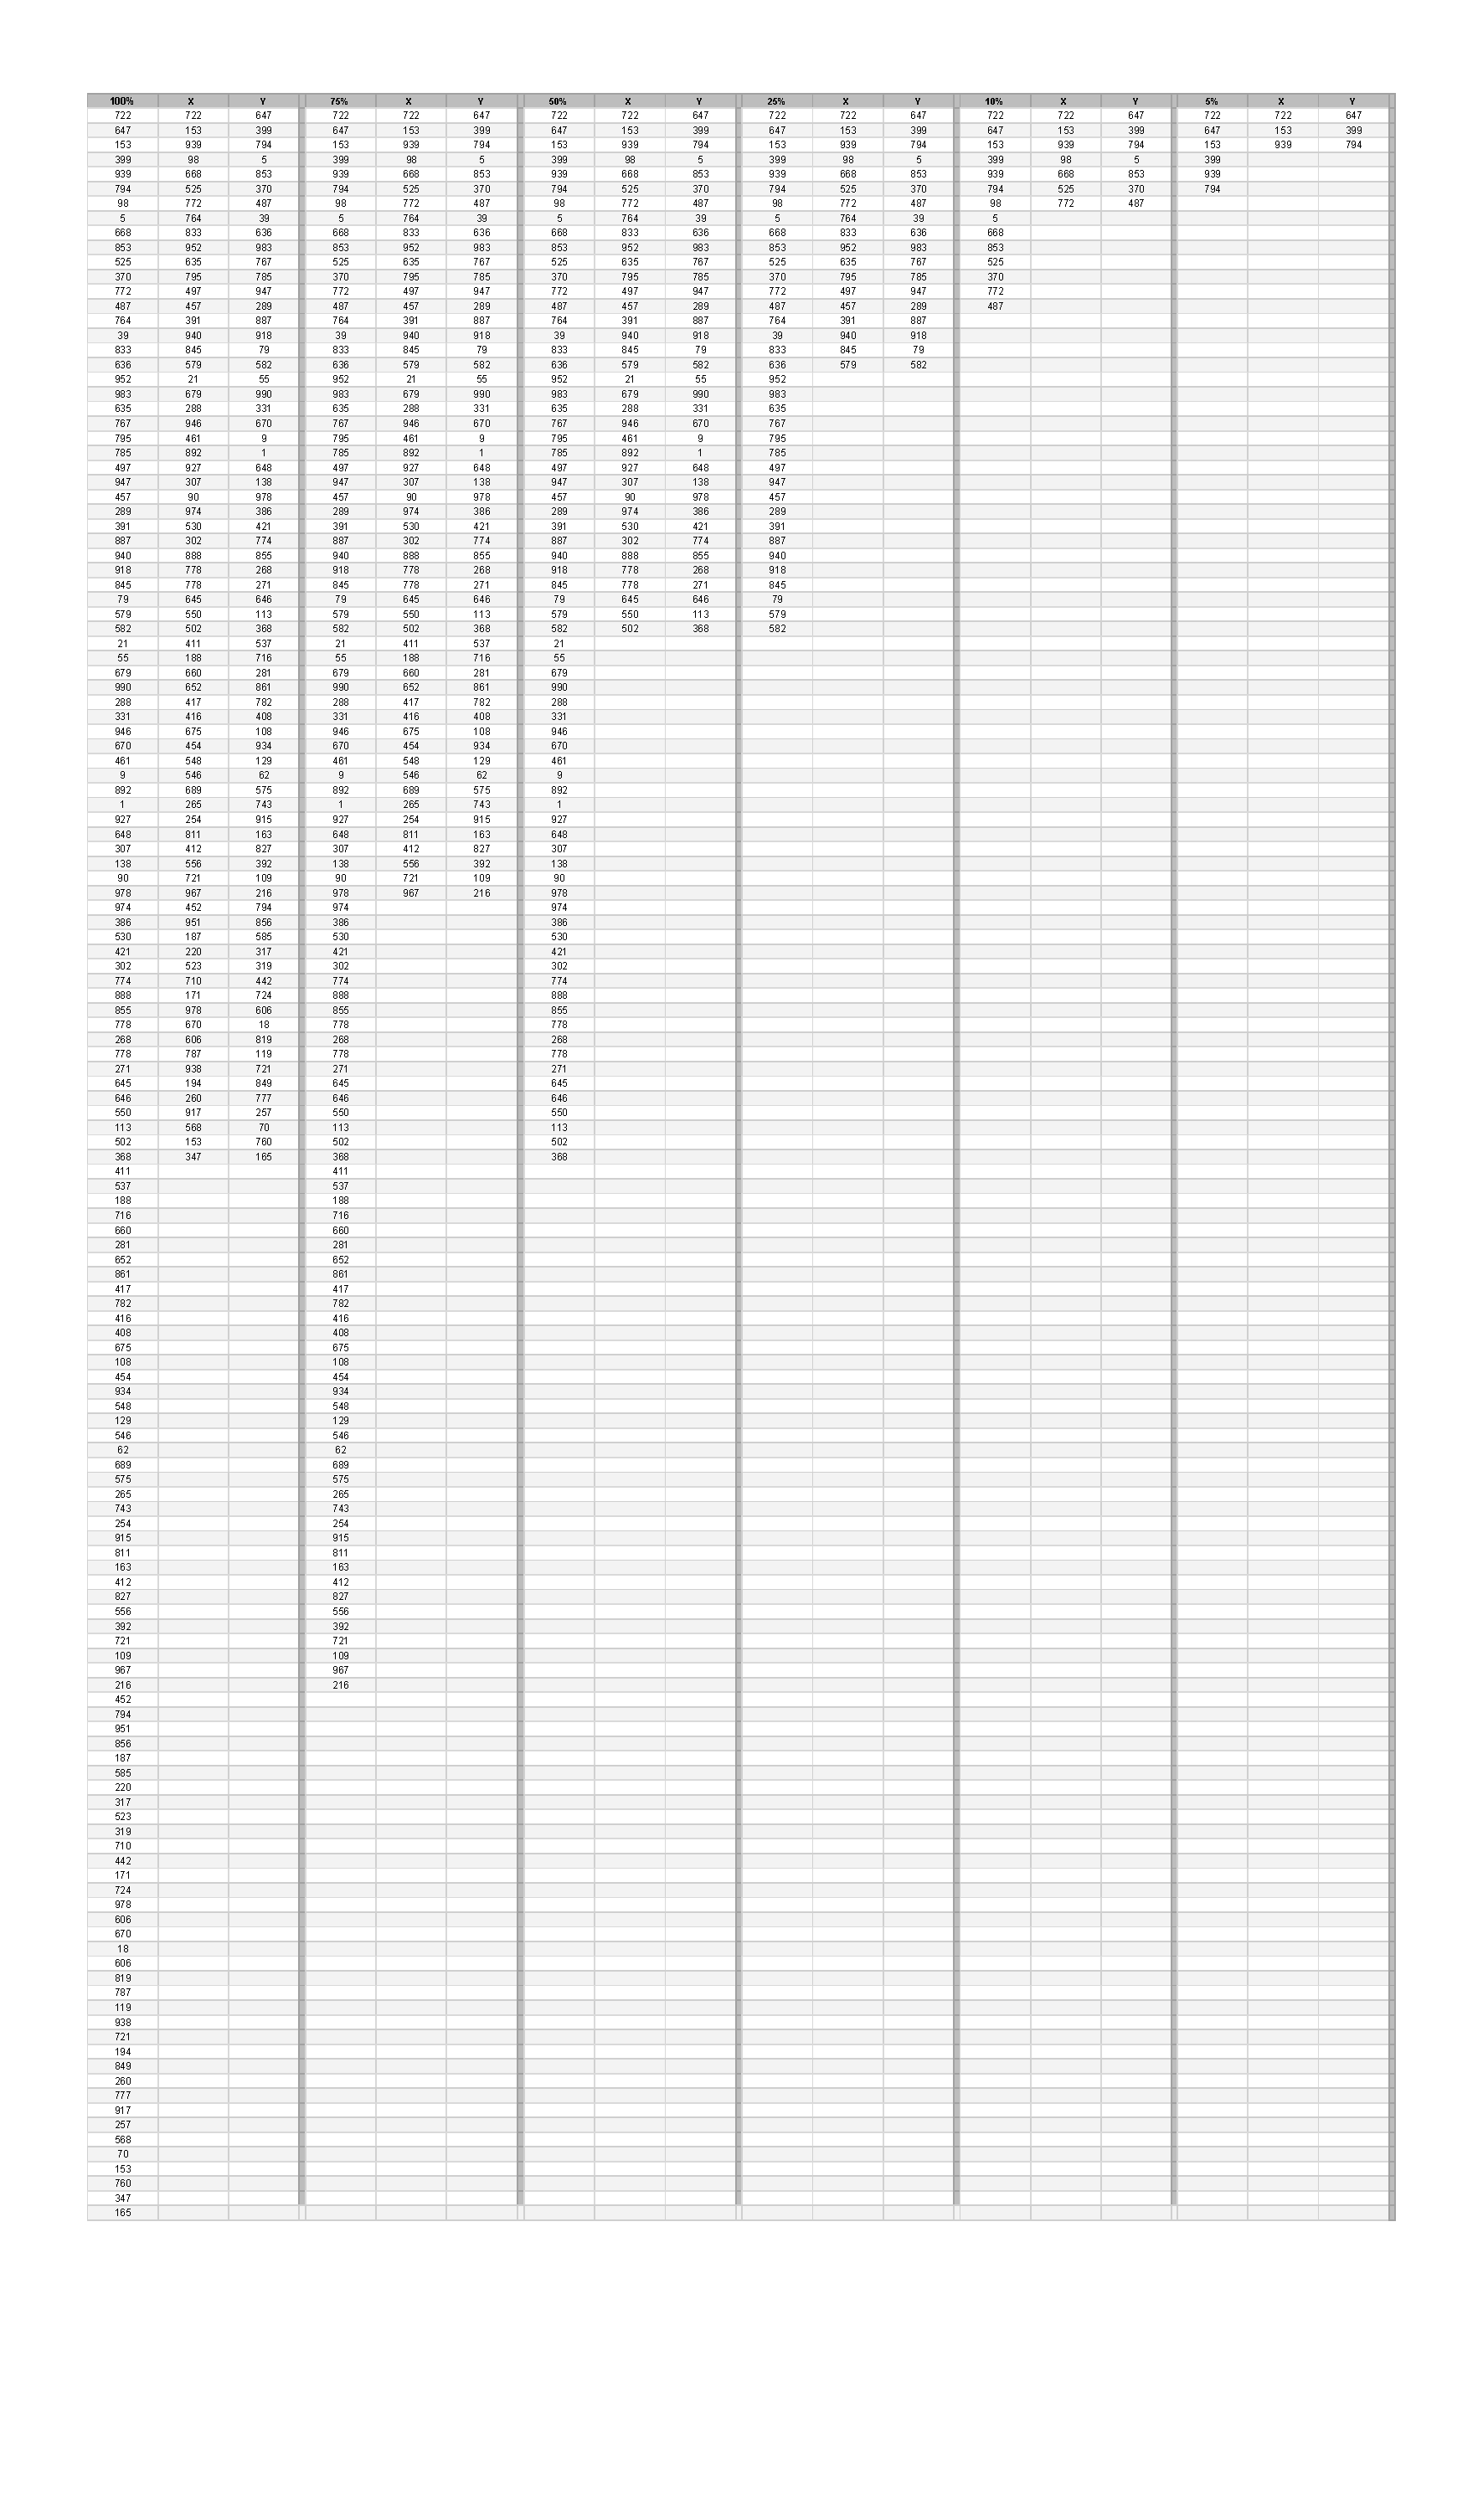
\includegraphics[width=0.74\textwidth]{tabelaRandJava.pdf}
                 \caption{Valores obtidos em um período}
                \label{fig:Desempenho}
        \end{figure}
       
Para a melhor compreensão de como é a aleatoriedade dos gráficos tanto o XorShift implementado, quanto o gerador do java, foi realizado gráficos em duas dimensões, com um par de coordenadas x e y, definido pelas seguintes periodicidades: 5\%, 10\%,25\%,50\%, 75\% e 100\%.

GRÁFICO EM XORSHIFT:

        \begin{figure}[H] 
            \centering
                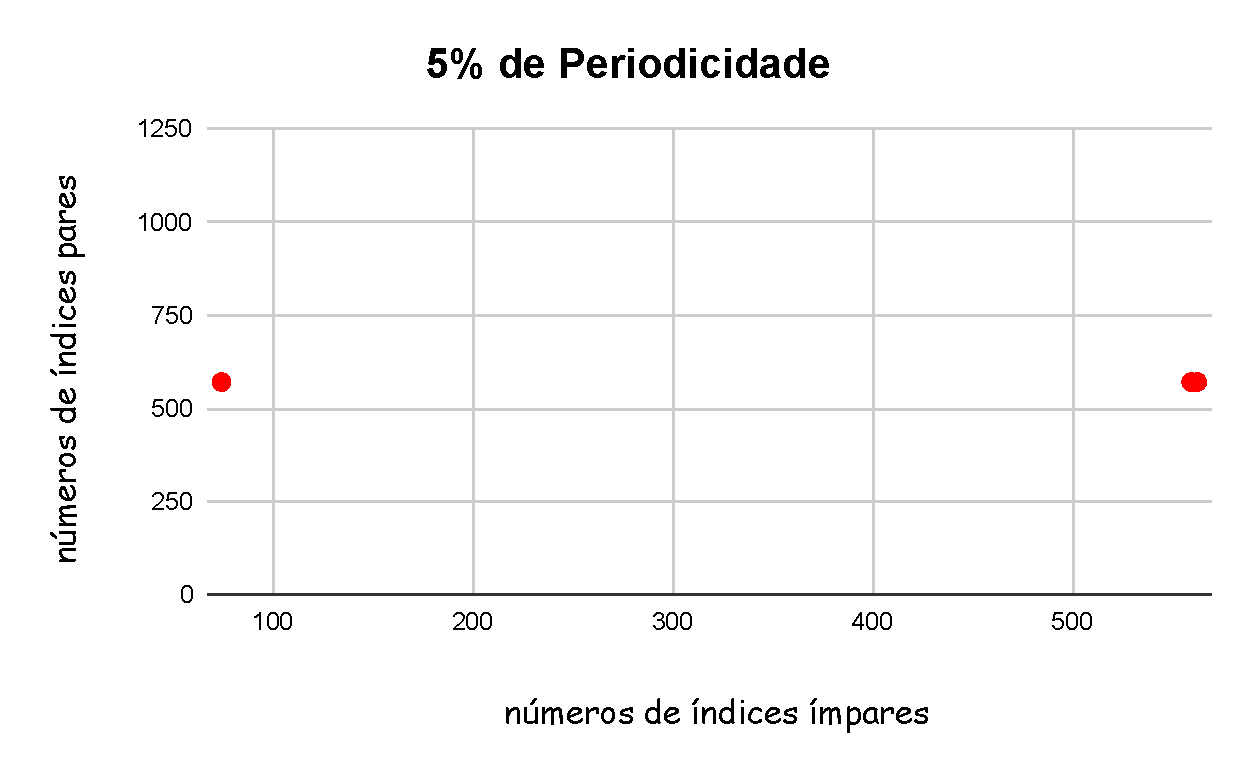
\includegraphics[width=0.496\textwidth]{5dePeriodicidade.pdf}
                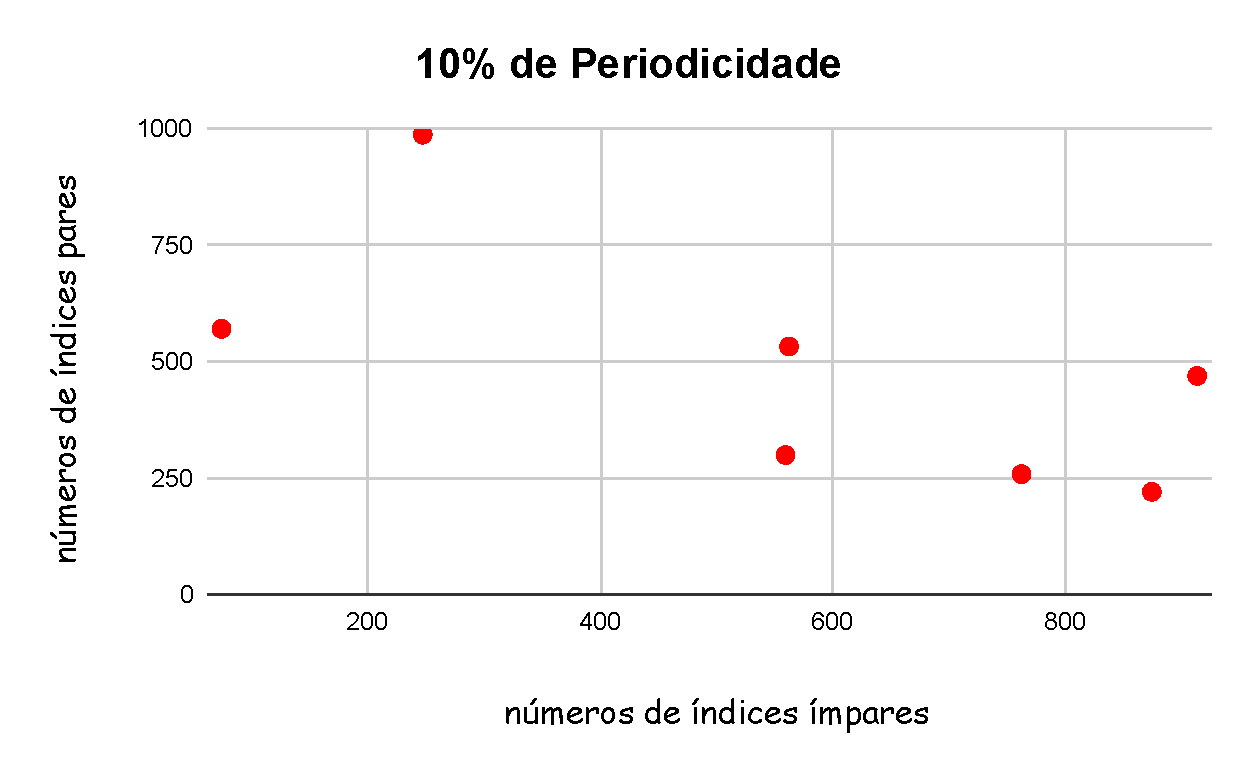
\includegraphics[width=0.496\textwidth]{10dePeriodicidade.pdf}
                \label{fig:Desempenho}
        \end{figure}
        
         \begin{figure}[H] 
            \centering
                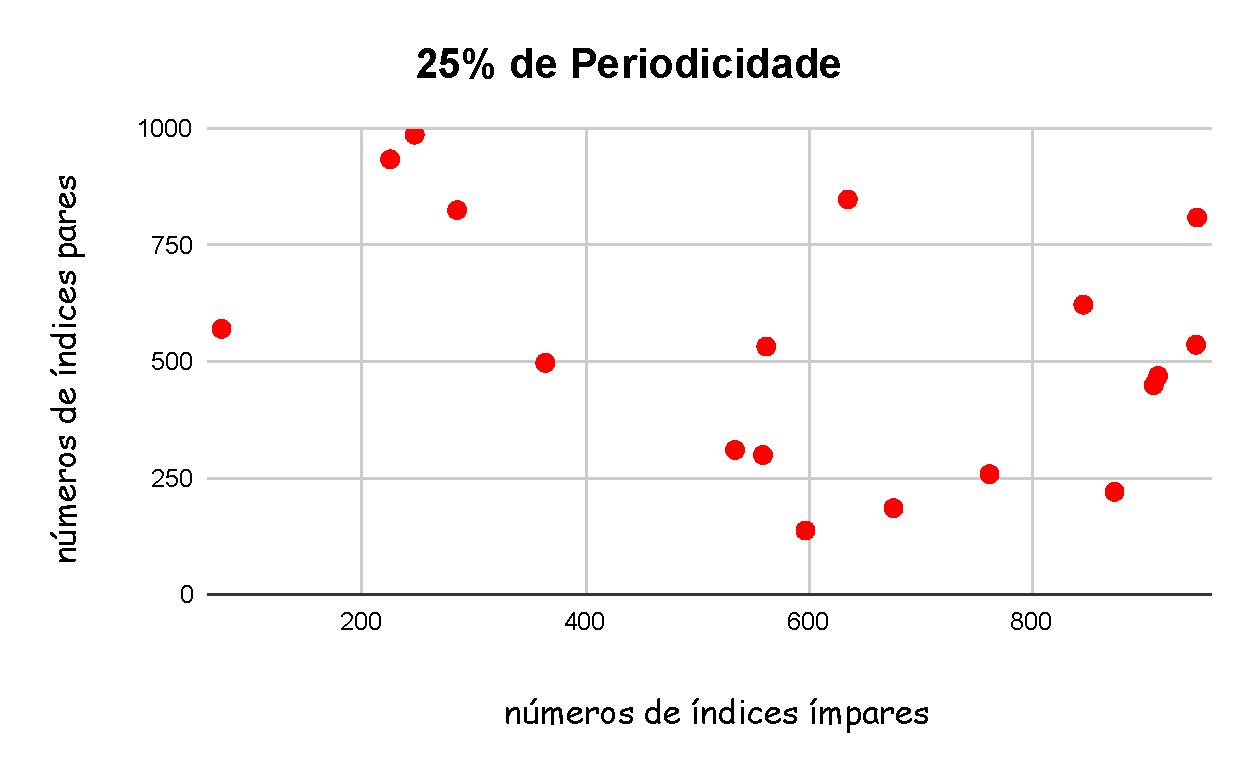
\includegraphics[width=0.496\textwidth]{25dePeriodicidade.pdf}
                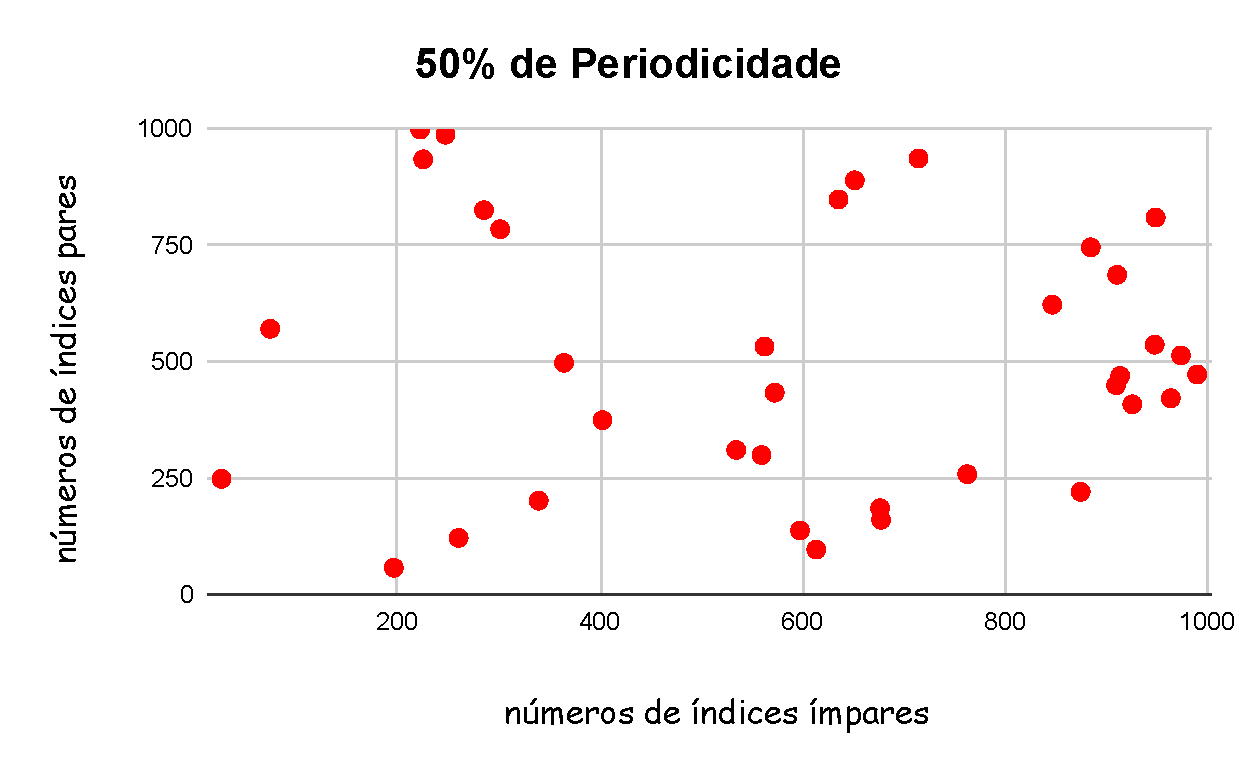
\includegraphics[width=0.496\textwidth]{50dePeriodicidade.pdf}
                     \label{fig:Desempenho}
        \end{figure}
        
         \begin{figure}[H] 
            \centering
                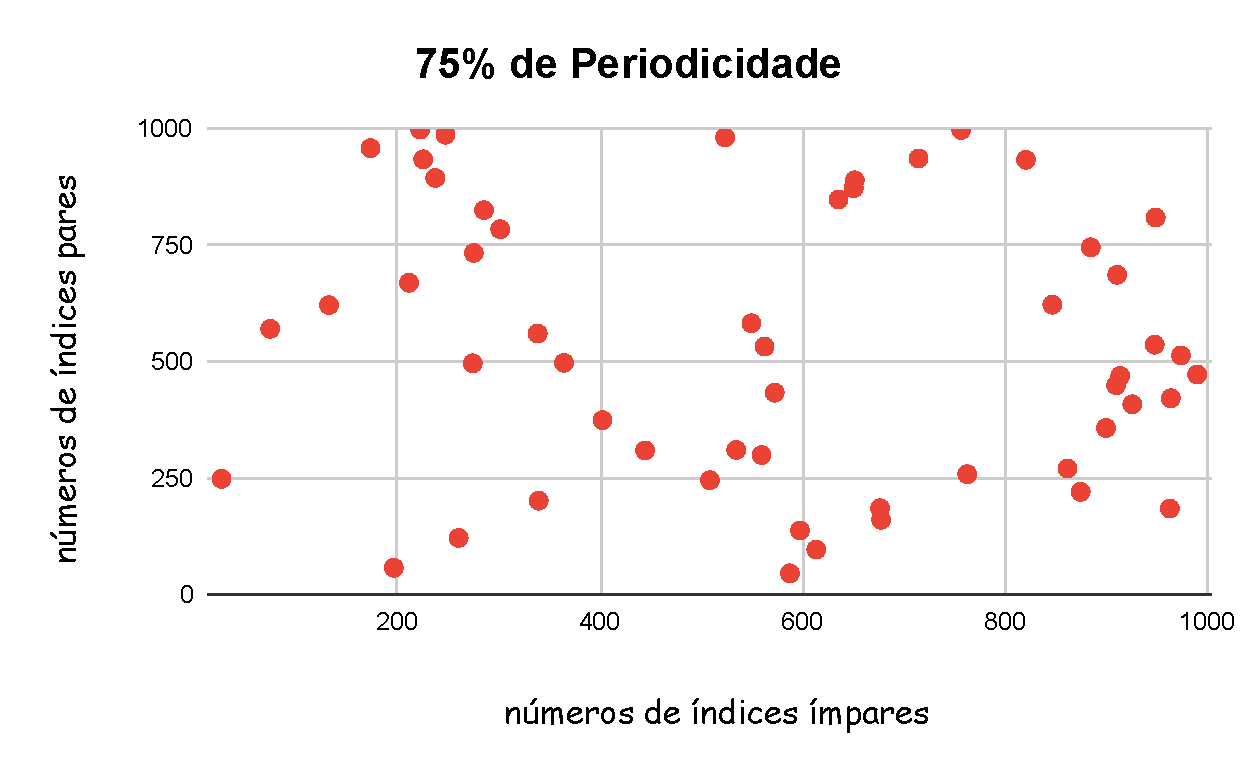
\includegraphics[width=0.496\textwidth]{75dePeriodicidade.pdf}
                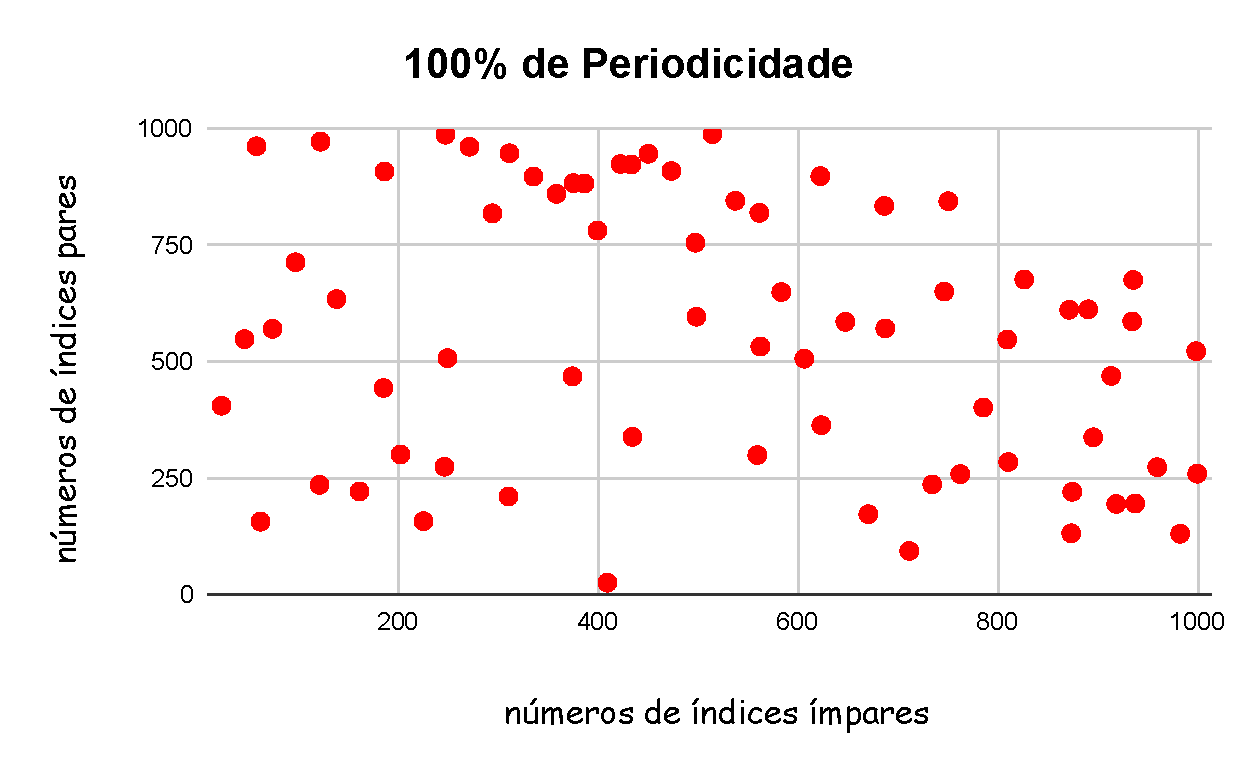
\includegraphics[width=0.496\textwidth]{100dePeriodicidade.pdf}    
                \label{fig:Desempenho}
        \end{figure}

\newpage
GRÁFICO EM JAVA:

  \begin{figure}[H] 
            \centering
                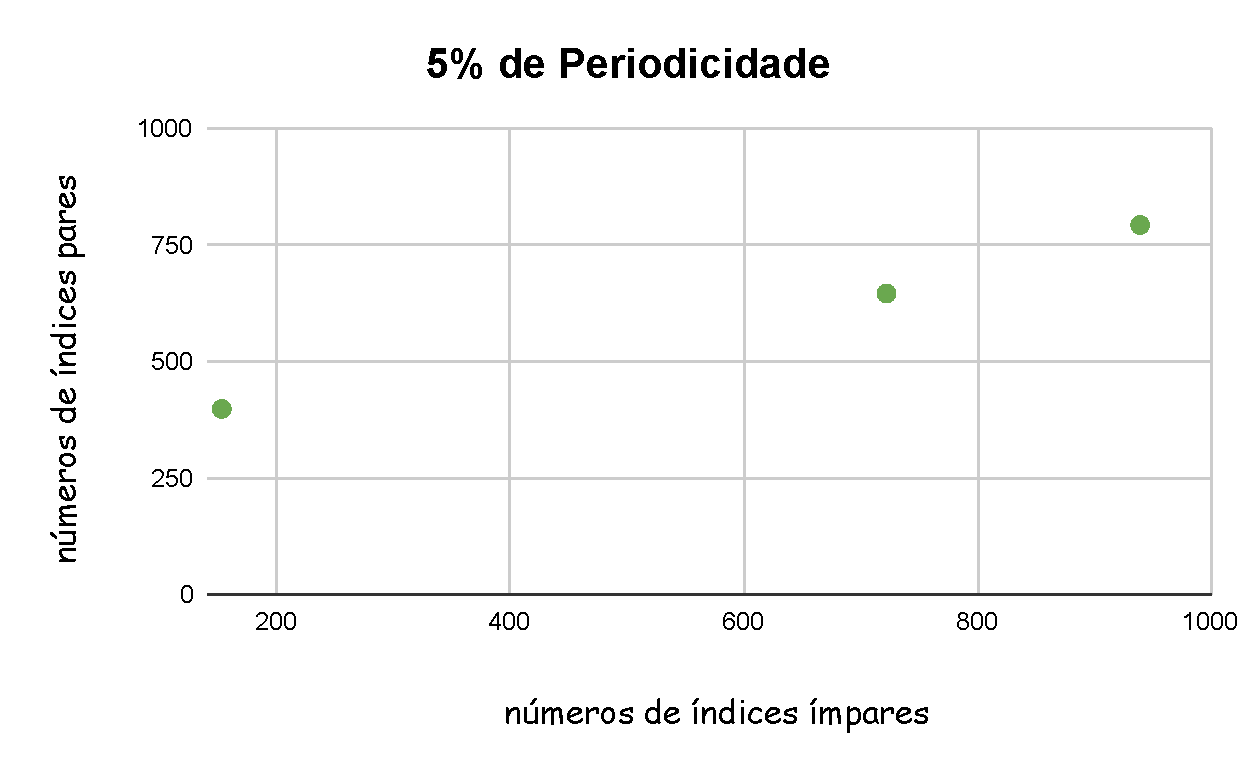
\includegraphics[width=0.496\textwidth]{5PeriodicidadeJ.pdf}
                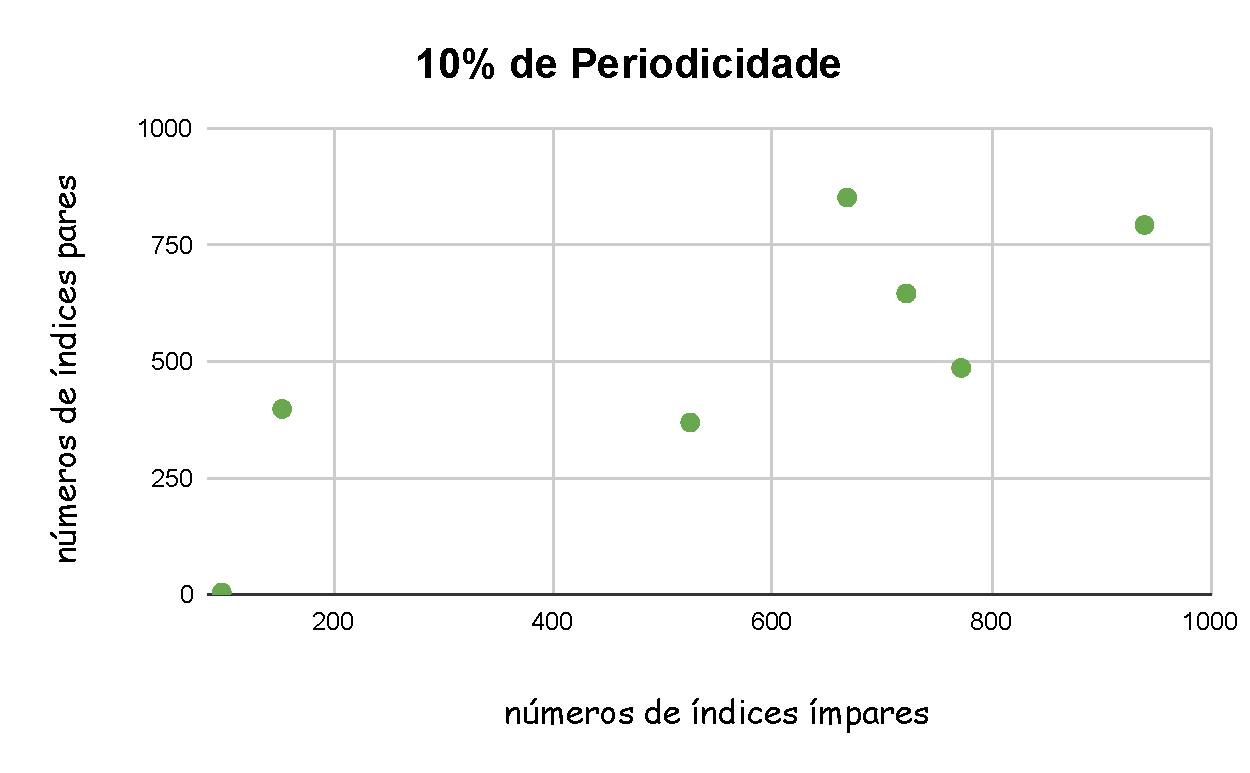
\includegraphics[width=0.496\textwidth]{10PeriodicidadeJ.pdf}
                 \label{fig:Desempenho}
        \end{figure}
          \begin{figure}[H] 
            \centering
                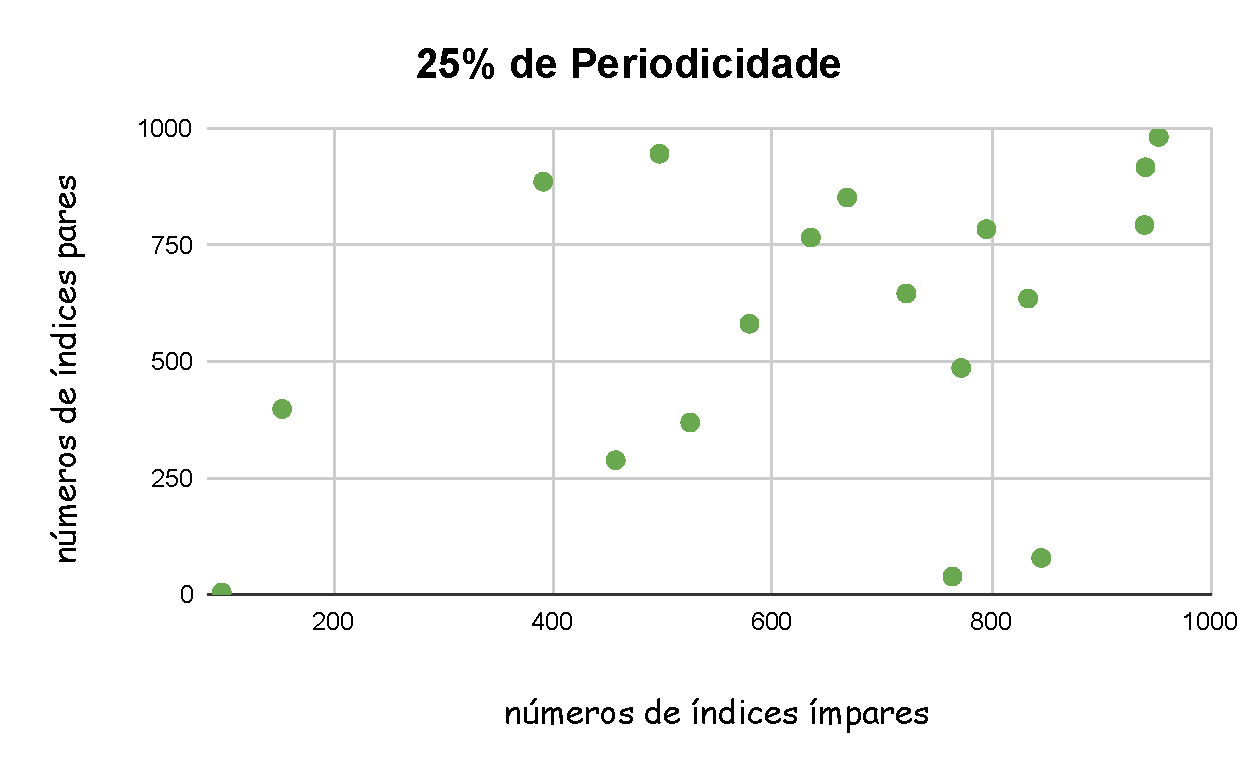
\includegraphics[width=0.496\textwidth]{25PeriodicidadeJ.pdf}
                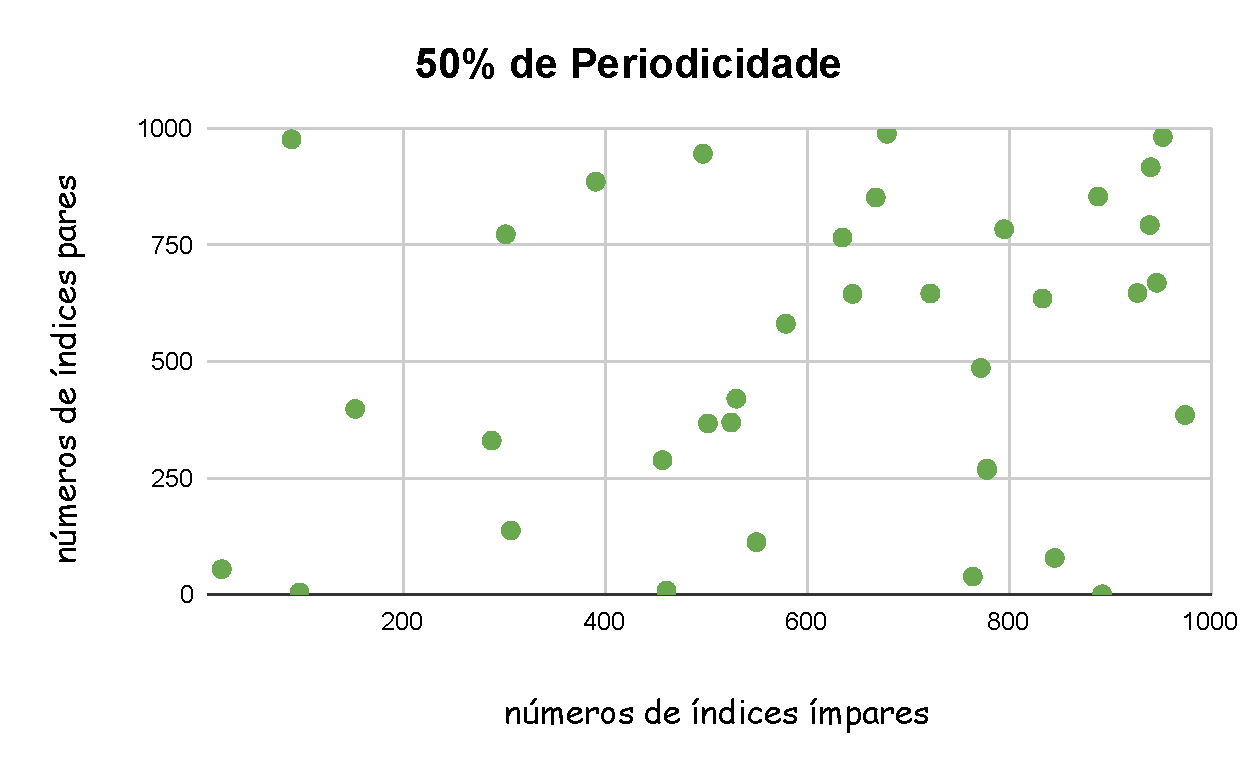
\includegraphics[width=0.496\textwidth]{50PeriodicidadeJ.pdf}
                 \label{fig:Desempenho}
        \end{figure}
          \begin{figure}[H] 
            \centering
                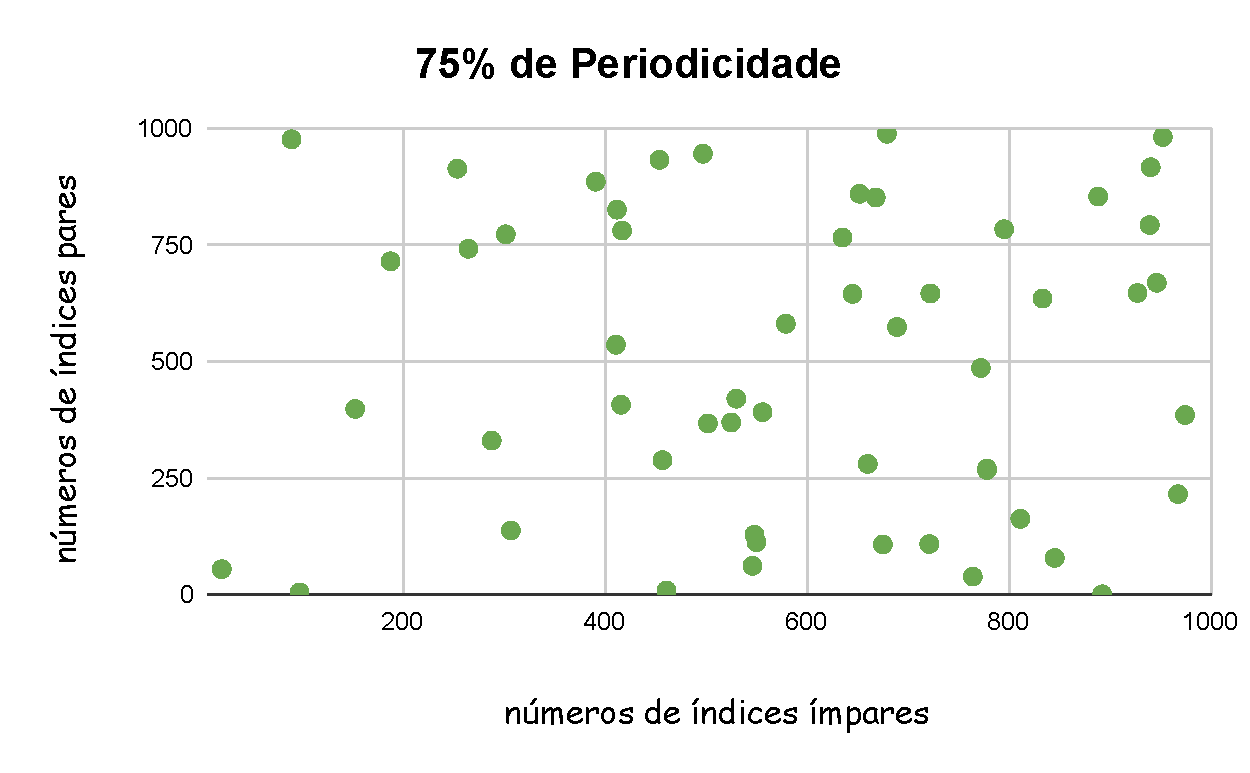
\includegraphics[width=0.496\textwidth]{75PeriodicidadeJ.pdf}
                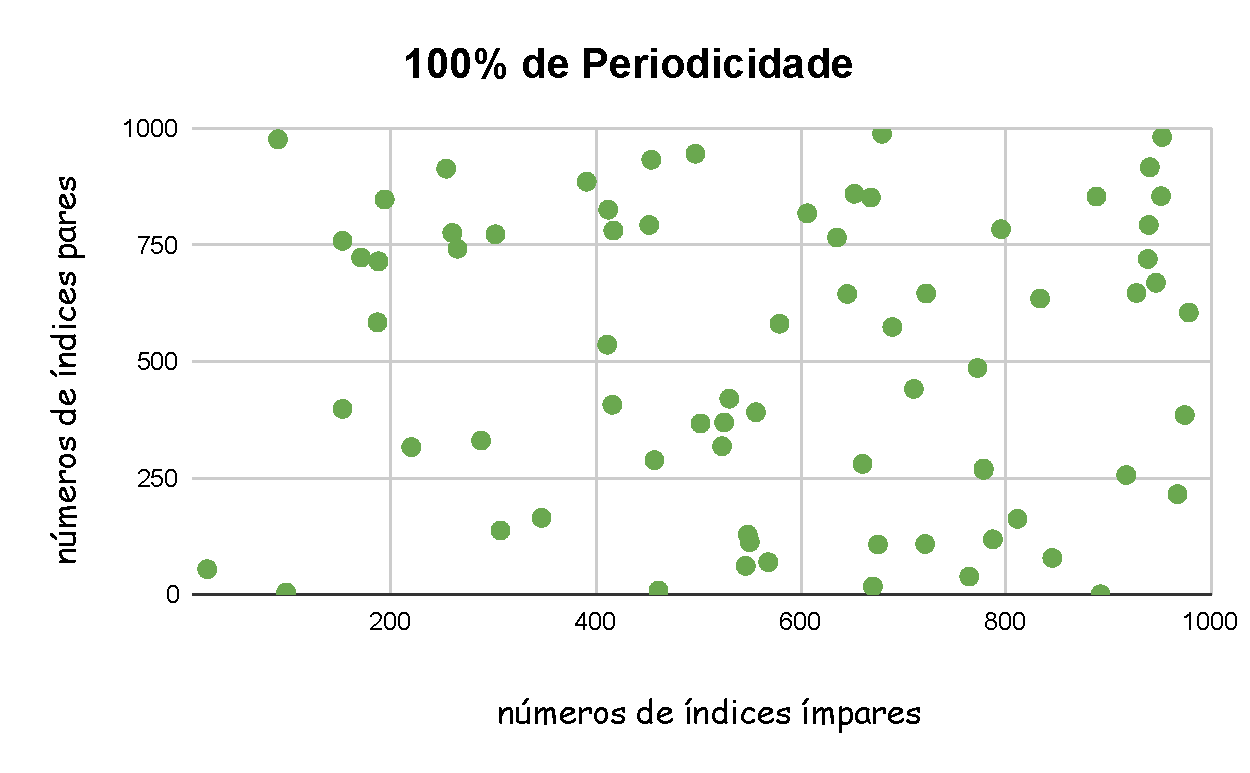
\includegraphics[width=0.496\textwidth]{100PeriodicidadeJ.pdf}    
                \label{fig:Desempenho}
        \end{figure}
        
Ao compilar os códigos, tanto o Xorshift elaborado,  quanto o Random do Java, pode-se perceber a aleatoriedade gerada por ambos, e a partir disso foi realizado os gráficos juntamente as tabelas com os devidos períodos, na execução das coordenadas,  foi empregue para os números em X os índices  ímpares da tabela - parte horizontal desta,  já para o Y os  índices pares da tabela - parte vertical desta. O gráfico do java.util.Random foi feito baseado no período do codigo xorshift, pois o período dele próprio seria grande demais.